\documentclass[notes]{subfiles}

\begin{document}
	\addcontentsline{toc}{section}{2.2 - The Derivative as a Function}
	\refstepcounter{section}
	\fancyhead[RO,LE]{\bfseries \large\nameref{cs22}} 
	\fancyhead[LO,RE]{\bfseries \currentname}
	\fancyfoot[C]{{}}
	\fancyfoot[RO,LE]{\large \thepage}	%Footer on Right \thepage is pagenumber
	\fancyfoot[LO,RE]{\large Chapter 2.2}

\section*{The Derivative as a Function}\label{cs22}
	\subsection*{Before Class}
	\addcontentsline{toc}{subsection}{Before Class}
	\subsubsection*{The Derivative as a Function}
	\addcontentsline{toc}{subsubsection}{The Derivative as a Function}
		\begin{ex}
			\begin{enumerate}[(a)]
				\item Use either method of the previous section to find the derivative of $f(x) = x^2 + 1$ at $(1,2)$.
					\vs{1}
					
				\item Find the derivative of $f(x)$ at $(2,5)$.
					\vs{1}
			\end{enumerate}
		\end{ex}
			
			
		\begin{defn}[The Derivative (as a Function)]
			The \textbf{derivative of a function} $f(x)$ is given as 
			\showto{ins}{
				\[\lim_{h\to 0} \dfrac{f(x+h) - f(x)}{h}\]
			}
			\showto{st}{
				\\ \vspace{.75in}
			}
			where $h$ is
			\showto{ins}{
				\fbox{a small change in $x$}.
			}
			\showto{st}{
				\blank{4}.
			}
		\end{defn}
			\newpage
			
		\begin{ex}
			\begin{enumerate}[(a)]
				\item Use the previous definition to compute $f'(x)$, if $f(x) = x^2 + 1$.  
					\vs{1}
				\item Find $f'(1)$ and $f'(2)$.
					\vs{.5}
			\end{enumerate}
		\end{ex}
		
	\subsubsection*{Differentiability \& Non-Differentiability}
\addcontentsline{toc}{subsubsection}{Differentiability \& Non-Differentiability}
		\begin{defn}[Differentiability]
			A function $f$ is \textbf{differentiable at }$a$ if 
			\showto{ins}{
				\fbox{$f'(a)$ exists}.
			}
			\showto{st}{
				\blank{3.5}. \\ \vspace{10pt}
			}
			It is \textbf{differentiable on an open interval} $(a,b)$ if it is 
			\showto{ins}{
				\fbox{differentiable at every number in the} \fbox{interval}.
			}
			\showto{st}{
				\blank{2.3} \\ \\ \blank{3}.
			}
		\end{defn}
		\begin{rmk}[A Note]
			Here is the formal definition of differentiability: a function $f(x)$ is differentiable at $a$ if 
			\showto{ins}{
				\[\lim_{h\to 0^-} \dfrac{f(x+h)-f(x)}{h} = \lim_{h\to 0^+} \dfrac{f(x+h)-f(x)}{h}\]
			}
			\showto{st}{
				\\ \\ \\ \\
			}
		\end{rmk}
			\newpage
			
		\begin{ex}
			Where is $f(x) = |x|$ differentiable?
		\end{ex}
			\vs{1}
			
		\begin{ex}
			Where is $g(x) = \llbracket x\rrbracket$ differentiable?
		\end{ex}	
			\vs{1}

		\begin{question}
			Rewrite the definition of continuity.  What relationship(s) do you see between continuity and differentiability?
		\end{question}
			\vs{1}
			
		\begin{rmk}[Differentiability vs. Continuity]
			\showto{ins}{
				If a function $f$ is differentiable, then it is continuous; the reverse is not true.
			}
			\showto{st}{
				\\[30pt]
			}
		\end{rmk}
			\newpage
			
		There are several characteristics which indicate that a graph is not differentiable at a point:
		\showto{ins}{
			\begin{itemize}
				\item A sharp corner
				\item A discontinuity
				\item A vertical tangent line
			\end{itemize}
		}
		\showto{st}{
			\begin{itemize}
			\setlength\itemsep{25pt}
				\item 
				\item
				\item
			\end{itemize}
		}
			\vs{.25}
		
	\subsubsection*{Other Notations}
	\addcontentsline{toc}{subsubsection}{Other Notations}
		\begin{rmk}
			\showto{ins}{
				\[f'(x) = y' = \dfrac{dy}{dx} = \dfrac{df}{dx} = \dfrac{d}{dx}[f(x)] = Df(x) = D_xf(x)\]
			}
			\showto{st}{
				\vspace*{1.5in}
			}
		\end{rmk}
		
		When we want to evaluate a derivative, we often use a vertical bar to communicate that we are evaluating.  If $f(x) = x^2$, then $f'(x) = 2x$, and $f'(1) = 2$; we could also notate this by writing
		\[\dfrac{dy}{dx}\bigg\rvert_{x = 1} = 2\]	
			\vs{1} \\
		\newsec $ $

	\subsubsection*{Pre-Class Activities}
	\addcontentsline{toc}{subsubsection}{Pre-Class Activities}
		\begin{ex}
			What are some similarities and differences between the definitions of the derivative in \S2.1 and the one in this section?
		\end{ex}
			\vs{1}
			\newpage
			
		\begin{ex}
			For any linear function $f(x) = ax + b$, $f'(x) = a$.  Try showing this with the formal definition of the derivative.  \emph{Without computation}, why would this be true?
		\end{ex}
			\vs{1}
			
		\begin{ex}
			Let $P$ represent the percentage of a city's electrical power that is produced by solar panels, $t$ years after January 1, 2015.
			\begin{enumerate}[(a)]
				\item What does $\dfrac{dP}{dt}$ represent in this context?  Include the units.
					\vs{.5}
					
				\item Convert the statement $\dfrac{dP}{dt}\bigg\rvert_{t = 3} = 2.1$ to an English sentence.
					\vs{1}
					
				\item Convert the English sentence into derivative notation: Five years after 2015, the percentage of a city's electrical power produced by solar panels was decreasing by 0.7 percent per year.
					\vs{.5}
					
			\end{enumerate}
		\end{ex}
		
		\begin{ex}
			The graph of a function $f$ is given.  State the input values at which $f$ is \emph{not} differentiable.\\
			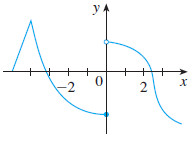
\includegraphics{2.2fig1}
		\end{ex}
			\newpage
			
		
	\subsection*{In-Class}
	\addcontentsline{toc}{subsection}{In-Class}
	\subsubsection*{Derivatives}
	\addcontentsline{toc}{subsubsection}{Derivatives}
		\begin{ex}
			Find a formula for $g'(x)$, if $g(x) = x^3 + 1$
		\end{ex}
			\vs{1}
			
		Even in this relatively benign example, the algebra got complicated.  Here are three algebraic reminders:
		\showto{ins}{
			\begin{itemize}
				\item $(x+a)^n\neq x^n + a^n$.  \emph{Please, do not make this mistake!}
				\item $(x+a)^2 = x^2 + 2ax + a^2$
				\item $(x+a)^3 = x^3 + 3x^2a + 3xa^2 + a^3$
			\end{itemize}
		}
		\showto{st}{
			\begin{itemize}
			\setlength\itemsep{25pt}
				\item 
				\item 
				\item 
			\end{itemize}
		}
			\vs{.25}
		
		\begin{rmk}[Four-Step Method]
			\showto{ins}{
				\begin{enumerate}[(1)]
					\item Write (and expand) $f(x+h)$.
					\item Subtract $f(x)$ from $f(x+h)$.
					\item Divide \#2 by $h$.
					\item Take the limit as $h\to 0$.
				\end{enumerate}
			}
			\showto{st}{
				\begin{enumerate}[(1)]
				\setlength\itemsep{25pt}
					\item 
					\item 
					\item 
					\item 
				\end{enumerate}
			}
		\end{rmk}
			\newpage
			
		\begin{ex}
			Use the four-step method to algebraically calculate $f'(x)$, if $f(x) = x^2 - 3x -1$.
		\end{ex}
			\vs{1}
			
		\begin{ex}
			Find $h'(x)$, if $h(x) = \sqrt{x}$
		\end{ex}
			\vs{2}
			
		The previous example gives rise to one of several common tips/tricks when algebraically calculating derivatives:
		\showto{ins}{
			\begin{itemize}
				\item Combine fractions
				\item Multiply by a conjugate
			\end{itemize}
		}
		\showto{st}{
			\begin{itemize}
			\setlength\itemsep{30pt}
				\item 
				\item 
			\end{itemize}
		}
			\newpage
			
		\begin{ex}
			Let $q(t) = \sqrt{1+t}$.  Show that $\dfrac{dq}{dt} = \dfrac{1}{2}(1+t)^{-1/2}$.
		\end{ex}
			\vs{1}
			
		\begin{ex}
			Let $k(x) = \dfrac{3+x}{x-2}$.  Find $k'(x)$.
		\end{ex}
			\vs{1.5}
			
	\subsubsection*{Slope Graphs}
	\addcontentsline{toc}{subsubsection}{Slope Graphs}
		\begin{ex}
			Use the graph of $f$ below to sketch the graph of $f'$.  
			\begin{center}
				\begin{tikzpicture}
					\begin{axis}[
						scale = 1.5,
						every tick label/.append style={font=\small},
						axis x line = middle,
						axis y line = middle,
			    			every axis y label/.style={at={(ticklabel cs:1.15)}},
			    			ytick = {0},
							y label style={at={(axis description cs:.2,1.15)},anchor=north},
			    			ylabel = {$f(x)$},
			    			ymin = -.5, ymax = 5,
		    				every axis x label/.style= {at ={(ticklabel cs:1)}},
		    				xtick = {1.13, 2.33, 3.53},
		    					x label style={at={(axis description cs:1.1,.1)},anchor=east},
		    				xlabel = {$x$},
		    				xmin = -1, xmax = 5
					]
						\addplot[thick, smooth,domain = -0.2:4.9] {.5*x^3-3.5*x^2+6*x+1.3};
						\coordinate (a1) at (1.13,4.33);
						\coordinate (a2) at (1.13,0);
						\coordinate (b1) at (2.33,2.6);
						\coordinate (b2) at (2.33,0);
						\coordinate (c1) at (3.53,0.86);
						\coordinate (c2) at (3.53,0);
					\end{axis}
					\draw[dashed] (a1)--(a2);
					\draw[dashed] (b1)--(b2);
					\draw[dashed] (c1)--(c2);
				\end{tikzpicture}	
			\end{center}

			\begin{center}
				\begin{tikzpicture}
					\begin{axis}[
						scale = 1.5,
						every tick label/.append style={font=\small},
						axis x line = middle,
						axis y line = middle,
			    			every axis y label/.style={at={(ticklabel cs:1.15)}},
			    			ytick = {0},
							y label style={at={(axis description cs:.2,1.15)},anchor=north},
			    			ylabel = {$f'(x)$},
			    			ymin = -.5, ymax = 5,
		    				every axis x label/.style= {at ={(ticklabel cs:1)}},
		    				xtick = {1.13, 2.33, 3.53},
		    					x label style={at={(axis description cs:1.1,.1)},anchor=east},
		    				xlabel = {$x$},
		    				xmin = -1, xmax = 5
					]
					\end{axis}
				\end{tikzpicture}
			\end{center}
		\end{ex}
			\newpage
			
		\begin{ex}
			Match the function in (a) - (d) with its derivative graph in (I) - (IV).  Give reasons for each choice.\\
			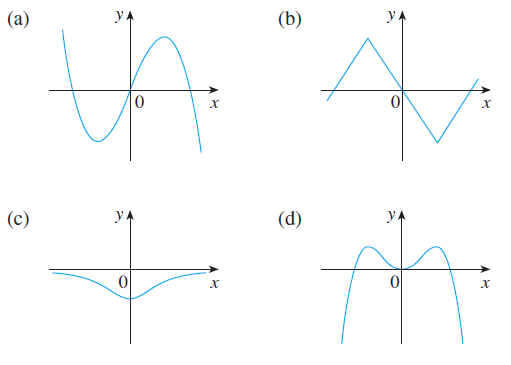
\includegraphics[width = .5\textwidth]{2.2fig2} 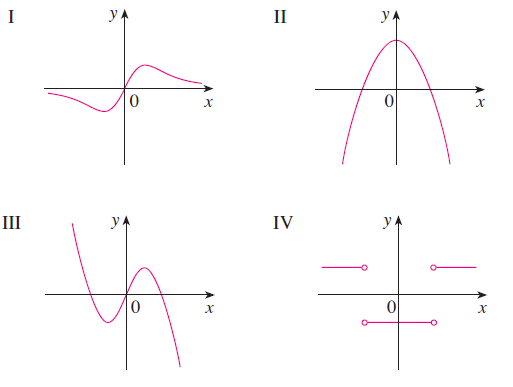
\includegraphics[width = .5\textwidth]{2.2fig3}
		\end{ex}
			\vs{1}
			
		\begin{ex}
			The graph of $g(t)$ is given.  Sketch a possible graph of $g'(t)$.
			\begin{flushleft}
				\begin{tikzpicture}
					\begin{axis}[
						axis x line = middle,
						axis y line = middle,
						every axis y label/.style={at={(ticklabel cs:1.1)}},
						y label style={at={(axis description cs:.5,1.1)},anchor=north},
						ylabel = {$g'(t)$},
						every axis x label/.style= {at ={(ticklabel cs:1)}},
						x label style={at={(axis description cs:1.1,.22)},anchor=east},
						xlabel = {$t$},
						xmin=-1,xmax=1,
						xtick = \empty,
						ytick = \empty
					]
					\addplot[thick, domain=-1:1,samples=100]{x^3-.5*x}; 
					\end{axis}
				\end{tikzpicture}
			\end{flushleft}
		\end{ex}
			\vs{1}
			\newpage
	
		\begin{ex}
			Consider the function $y=ax-a$.  Find $\dfrac{df}{dx}$ and $\dfrac{df}{da}$.
		\end{ex}
			\vs{1}

	\subsubsection*{Higher Derivatives}
	\addcontentsline{toc}{subsubsection}{Higher Derivatives}
		In physics, higher-order derivatives are very important.  If $s(t)$ is a position function, then the first derivative $s'(t)$ is called the \emph{velocity}, often written as $v(t)$.  The second derivative of position (so, the first derivative of velocity) is called \emph{acceleration}, often written as $a(t)$.  The third derivative also has a special name, called the \emph{jerk}, $j(t)$.
		\begin{rmk}[Notation for Higher-Order Derivatives]
			\showto{ins}{
				\begin{itemize}
				\setlength\itemsep{5pt}
					\item Second derivative: $f''(x)$, $\dfrac{d^2y}{dx^2}$
					\item Higher Derivatives: $f^{(n)}(x)$, $\dfrac{d^ny}{dx^n}$ 
				\end{itemize}
			}
			\showto{st}{
				\begin{itemize}
				\setlength\itemsep{25pt}
					\item Second derivative: 
					\item Higher Derivatives: 
				\end{itemize}
			}
		\end{rmk}
	
		\begin{ex}
			If $f(x) = x^3-x$, find $f''(x)$, $\dfrac{d^3f}{dx^3}$, and $f^{(4)}(x)$.
		\end{ex}		
			\vs{2}
			\newpage
	
	\subsection*{After Class}	
	\addcontentsline{toc}{subsection}{After Class}
		\begin{ex}
			Find the first two derivatives of $a(x) = \sqrt{9-x}$.  Write your answer using both notations for the derivative.
		\end{ex}	
			\vs{2}
			
		\begin{ex}
			The graph of $f$ is given.  Sketch a possible graph for $f'$.  \\
			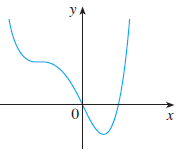
\includegraphics[scale = 1.2]{2.2fig4}
			\vs{.75}
		\end{ex}
	\clearpage
\end{document}